\documentclass{article}
\newcommand\tab[1][1cm]{\hspace*{#1}}
\usepackage[margin=60pt]{geometry}
\usepackage[utf8]{inputenc}
\usepackage{hyperref}
\usepackage{makeidx}
\usepackage{graphicx}
\graphicspath{{./res/}}
\makeindex
\begin{document}
\begin{titlepage}
   \vspace*{\stretch{1.0}}
   \begin{center}
      \Huge\textbf{IoT Project: "Keep your distance"}\\
      \vspace{5mm} %5mm vertical space
      \Large Prof. Matteo Cesana - Year 2020/2021\\
      \vspace{5mm} %5mm vertical space
      \large\textit{Gabba Rohit [codice persona: 10706944]}
      \\
      \large\textit{Tortorelli Giuseppe [codice persona: 10582962]}
   \end{center}
   \vspace*{\stretch{2.0}}
\end{titlepage}
\printindex

\section{TinyOS}
In order to keep track of the consecutive messages we decided to identify them with an incremental identifier. \\\\
The message struct is composed of the fields:
\begin{itemize}
   \item \textit{id}: the id of the sender mote
   \item \textit{msg\_number}: the id of the message sent from that mote
\end{itemize}
We decided to assign three arrays of fixed length to each mote:
\begin{itemize}
   \item \textit{near\_motes\_ids}: to save the id numbers of the near motes
   \item \textit{near\_motes\_counters}: to save the number of consecutive messages received from that mote
   \item \textit{near\_motes\_msgs\_number}: to save the id number of the message that we expect to receive from that mote
\end{itemize}
Every time a mote sends a message, the id to be assigned to the message is incremented.\\
At the receiving end of a message, the \textit{near\_motes\_ids} array is scaned to find the id of the sender mote.\\\\
If the the Id is not found then it is added to the first spot available in the array; otherwise we procede by checking the id of the message received.\\\\
We compare the expected id number from \textit{near\_motes\_msgs\_number} array with the value received from the mote. If the two values don't match then the counter that keeps track of the consecutive messages is restarted with the value 1.\\\\
Otherwise check the value of the \textit{near\_motes\_counters} array: if 10 consecutive messages have been received then an alarm is launched and the counter is restarted, otherwise the counter is incremented.


\section{Cooja}
We tested the functioning of the system by simulating it in \textit{Cooja} with 5 \textit{Sky mote}s and trying various configurations.\\\\
During the simulation we assumed that the messages are received without any interferences, therefore we ignored the cases where the counter is automatically reset because of a non correct delivery of a message.
\\\\
Here are some screenshots of the configuration tried during the simulation (ordered as in the log file)
\\
\begin{center}
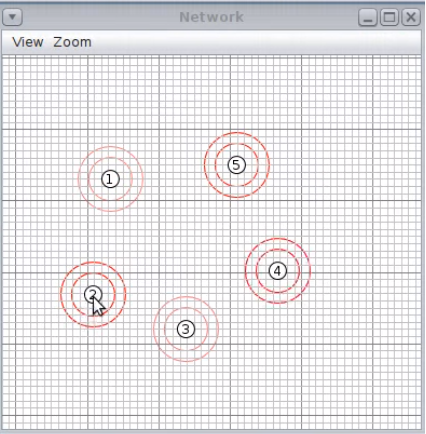
\includegraphics[scale=1]{img1.png}
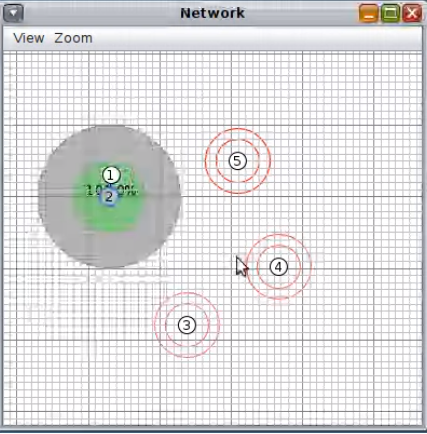
\includegraphics[scale=1]{img2.png}
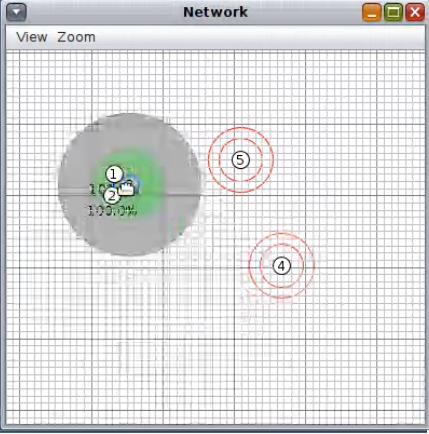
\includegraphics[scale=1]{img3.png}
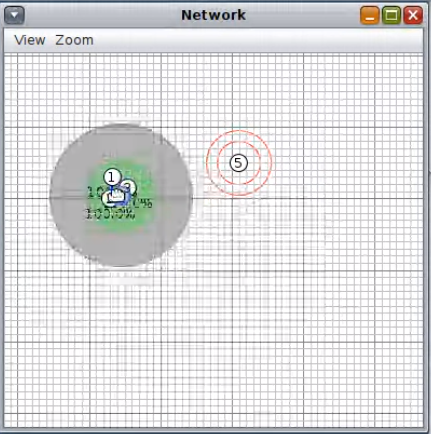
\includegraphics[scale=1]{img4.png}
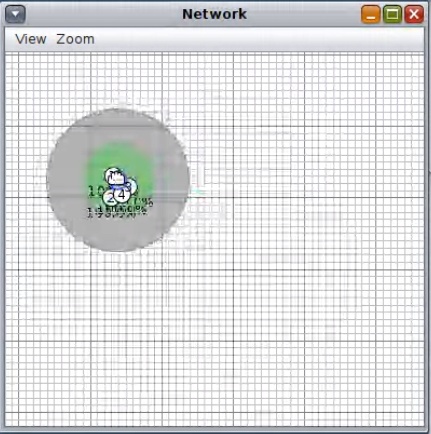
\includegraphics[scale=1]{img5.png}
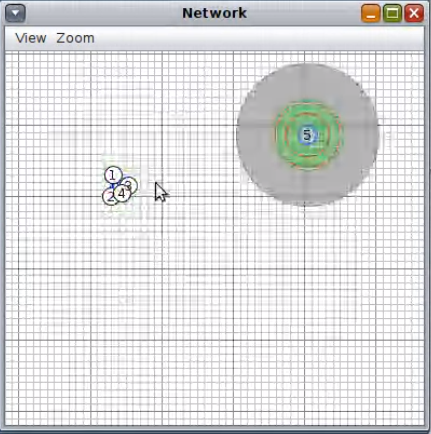
\includegraphics[scale=1]{img6.png}
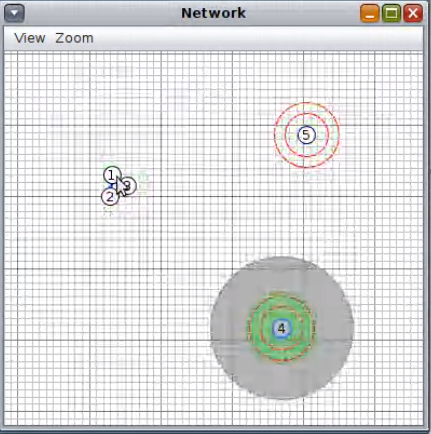
\includegraphics[scale=1]{img7.png}
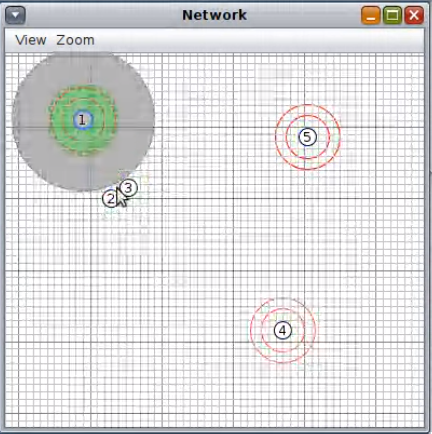
\includegraphics[scale=1]{img8.png}
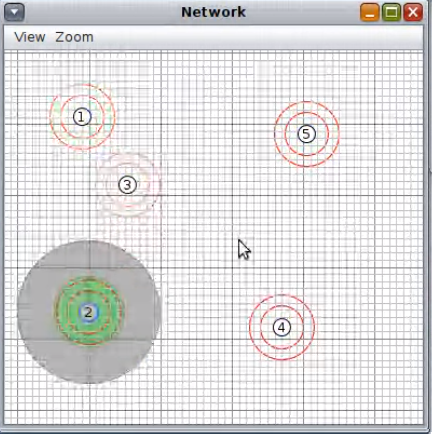
\includegraphics[scale=1]{img9.png}
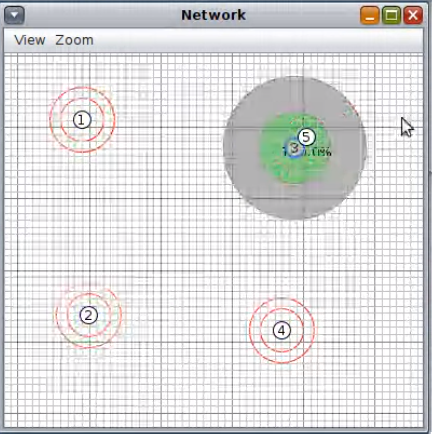
\includegraphics[scale=1]{img10.png}
\end{center}
We have assigned a socket to each mote with a different port number (from 6001 to 6005) towards the ip of \textit{Node-RED}.


\section{Node-RED}

We created 5 (number of motes chosen for the simulation) \textit{tcp in} nodes, each of them listening on the port of the associated mote.\\
Then we used the \textit{function} node to filter the alarm messages from the log sent by \textit{Cooja} and extract the Ids of the involved motes.\\
Finally we used the \textit{htttp request} node to send a POST request towards \textit{IFTTT} by specifying our API key.

\section{IFTTT}
Once received the messages through a \textit{Webhooks} applet listening on the \textit{ALARM} event,
we sent a notification on \textit{IFTTT} app for the cellular phone containing the message:\\\\
\textit{"ALARM mote x: I'm close to mote y! COVID"}\\\\
Wheree \textit{x} is the id of the mote that sent the alarm.

\end{document}